\documentclass[]{article}
\usepackage{kotex}
\usepackage{subcaption}
\usepackage{graphicx}
\usepackage{adjustbox}
\usepackage{booktabs}
\usepackage{comment}
\usepackage{amssymb} % math
\usepackage{multirow}
\usepackage{hyperref}
\usepackage{mathtools}%화살표 위 문자 삽입
\usepackage{amsmath}
\usepackage{multirow}

\newtheorem{definition}{Definition}

% Keywords command
\providecommand{\keywords}[1]
{
	\small	
	\textbf{\textit{Keywords---}} #1
}


%opening
\title{Conditional Generative Adversarial Network-based Travel Route Recommendation}


\author{
	\textit{Sunbin Shin \href{https://orcid.org/0009-0001-9440-5249}{
\includegraphics[scale=0.5]{fig/ORCIDiD_icon16x16.png}}} \\
	\textit{Yu Seung Kang \href{https://orcid.org/0009-0000-1465-4097}{
\includegraphics[scale=0.5]{fig/ORCIDiD_icon16x16.png}}} \\
	\textit{Jason J. Jung \href{https://orcid.org/0000-0003-0050-7445}{
\includegraphics[scale=0.5]{fig/ORCIDiD_icon16x16.png}}} \\ \and \newline 
	Department of Computer Engineering, Chung-Ang University \and \newline 84 Heukseok-ro, Seoul, 06974, Korea \and
	\textbf{\{defendsunbin, kangusng, j3ung\}@cau.ac.kr}
}


\begin{document}
	
	\maketitle

\begin{abstract}
In this study, we propose a route recommendation model using a Conditional Generative Adversarial Network (CGAN), based on the extraction of user characteristics and route features. Tourist routes have unique attributes distinct from traditional products like movies or books. To overcome this, we extract features from the relationship between users and routes, including locations, and the route characteristics represented by the sequence of places, thereby constructing a latent vector. We train the CGAN using the latent vector and user preference data for routes to address the data sparsity issue in the relationship between routes and users. The generated samples are then used to predict user route preferences. To evaluate the effectiveness of our proposed model, we employ real-world tourist route datasets. 

Experimental results show that our model records up to approximately 239.36\% improvement in Mean Absolute Error (MAE) and 108.72\% in Root Mean Squared Error (RMSE) compared to the best-performing models. Additionally, in further experiments conducted in sparse data environments, our model demonstrates adaptability with about 197.34\% and 107.86\% improvements in MAE and RMSE, respectively, compared to the best-performing models, thereby confirming its efficacy in sparse data situations.
\end{abstract}

\keywords{Recommender System, Heterogenous Information Network, RNN, MLP, Conditional Generative Adversarial Network}

\section{Introduction}
\label{sec:Intro}

Tourism is one of the largest industries in the world, and with this trend, online travel agencies (OTAs) like Expedia, Klook, and TripAdvisor have emerged to continuously provide online services. However, with the introduction of a variety of tourism products, the amount of tourist information has become overwhelming, making it difficult for users to quickly find products of interest among the vast array of tourism information.
\begin{figure}[!htbp]
	\centering
	\begin{subfigure}[b]{0.45\textwidth}
		\centering
		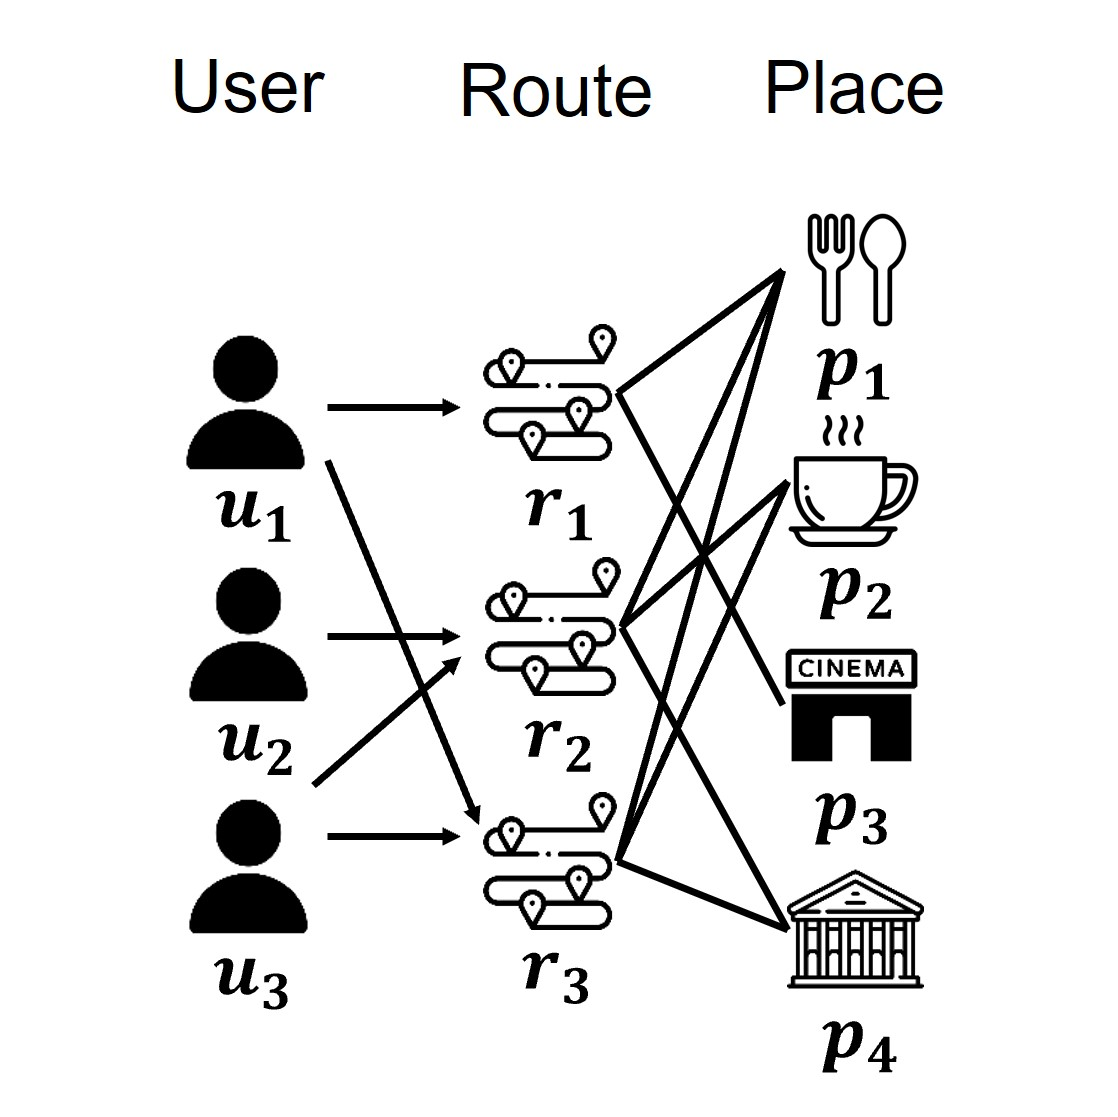
\includegraphics[width=\textwidth]{fig/그림1.jpg}
		\caption{Example of HIN}
		\label{fig1:image1}
	\end{subfigure}
	\hfill
	\begin{subfigure}[b]{0.45\textwidth}
		\centering
		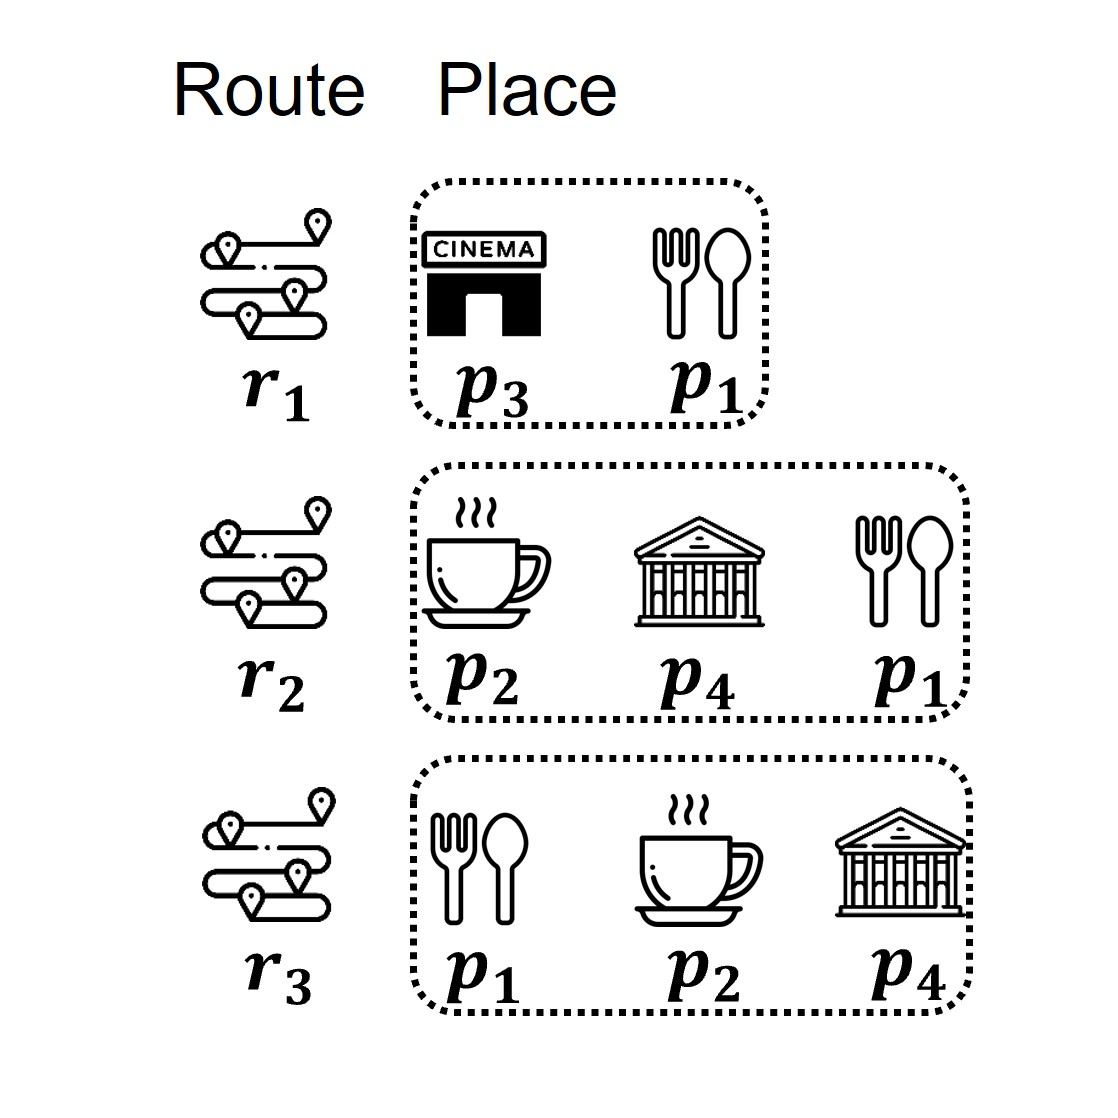
\includegraphics[width=\textwidth]{fig/그림2.jpg}
		\caption{Example of Route Sequence}
		\label{fig1:image2}
	\end{subfigure}
	\caption{Example of HIN and Route.}
	\label{fig1}
\end{figure}

\begin{comment}
	\begin{figure}[!htbp]
		\centering
		\begin{subfigure}[b]{0.45\textwidth}
			\centering
			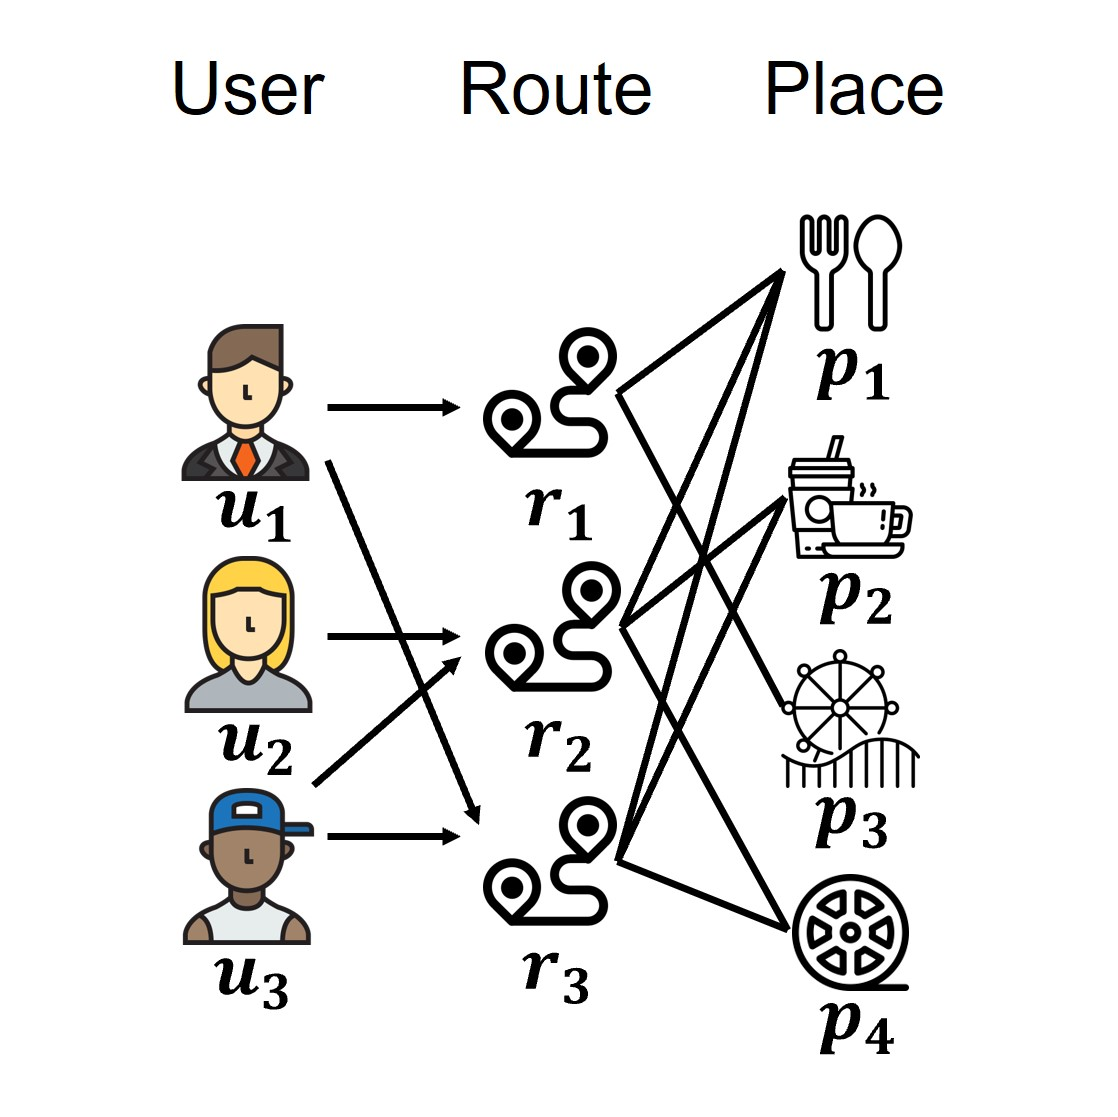
\includegraphics[width=\textwidth]{fig/HIN_example.jpg}
			\caption{Example of HIN}
			\label{fig1:image1}
		\end{subfigure}
		\hfill
		\begin{subfigure}[b]{0.45\textwidth}
			\centering
			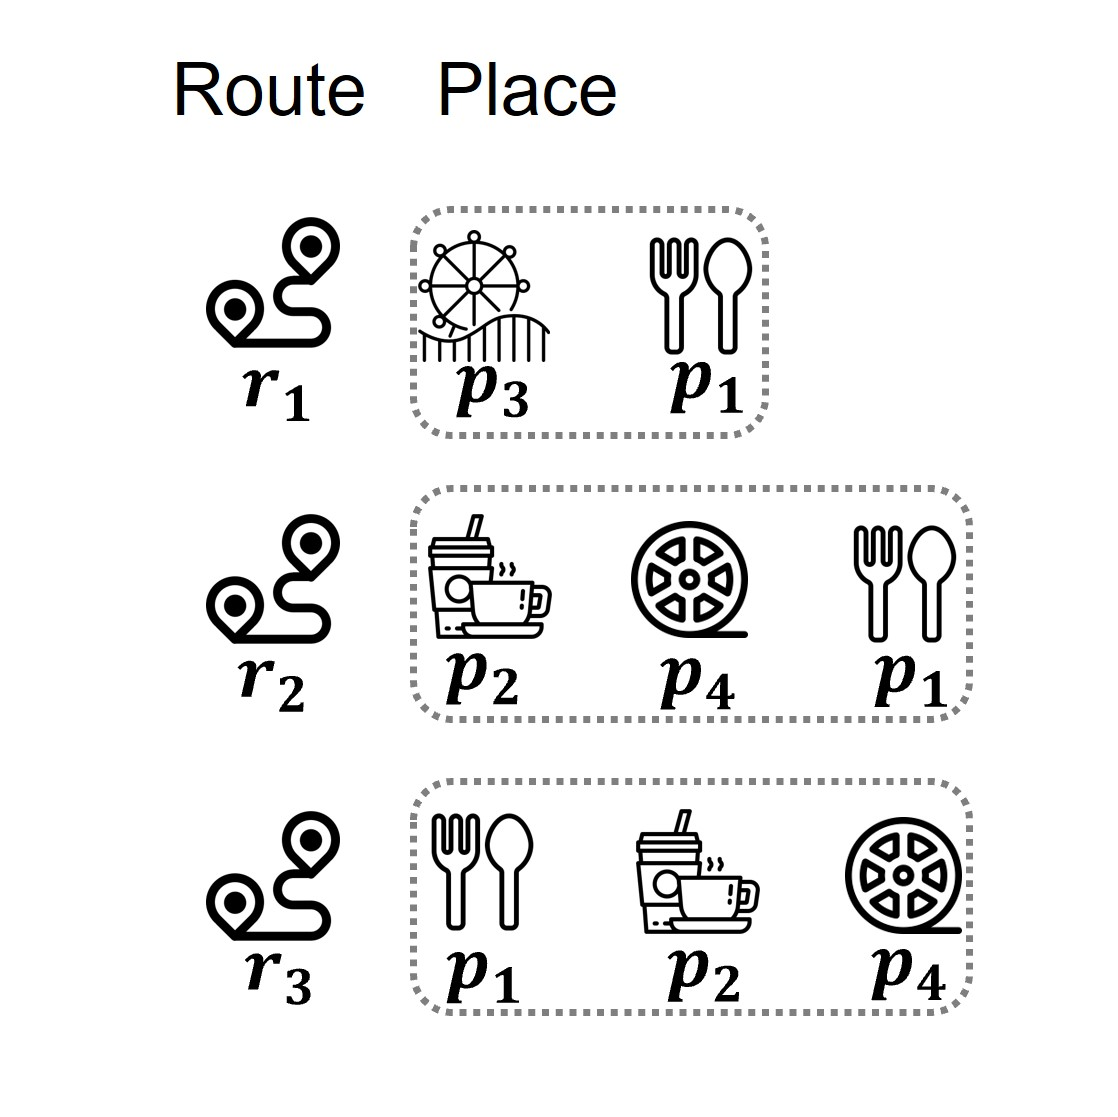
\includegraphics[width=\textwidth]{fig/RNN_example.jpg}
			\caption{Example of Route Sequence}
			\label{fig1:image2}
		\end{subfigure}
		\caption{Example of HIN and Route.}
		\label{fig1}
	\end{figure}...
\end{comment}


A travel route recommendation system is an important tool for addressing the problem of information overload in tourism. However, compared to traditional items such as books, food, and movies, travel recommendations have unique characteristics. These characteristics pose significant challenges in designing a systematic and flexible recommendation framework for personalized travel product recommendations. 

Firstly, travel data is sparser than traditional products. Travel requires time and financial cost. Users typically don't spend much time on travel websites, and the probability of encountering and evaluating travel routes is lower compared to the cost of watching a movie. 

Secondly, routes are composed of places. To learn the relationship between users and routes and extract user features, not only users and routes but also places need to be included. For example, based on the type of places that a user frequently visits (e.g., cafés, cinemas, museums), routes including similar places can be recommended.

Thirdly, routes can be represented by a sequence of places, and users may define routes composed of the same places but in different orders with different routes. For example, in Fig. 1(b), two routes composed of the same places can be defined as different routes depending on the user. Therefore, this sequence, i.e., the sequence of places, is one of the important features of a route.

Various studies have proposed to recommend customized travel packages. The PersonalTour, a multi-agent recommendation system, was proposed to find suitable travel products based on user preferences \cite{6040800}. To distinguish travel packages from conventional recommendation items and analyze these features, the Tourism-Region-Season-Theme (TAST) model was introduced. Additionally, an extension of the TAST model, the Tourist-Relationship-Area-Season-Theme (TRAST) model, was proposed to capture potential relationships between tourists within each travel group \cite{6365185}. Yu et al. suggested using location-based social networks to recommend personalized travel products, utilizing data collected from users' social networks and employing a collaborative filtering approach to derive destination preferences \cite{7145457}.

This paper proposes a travel route recommendation model that considers the characteristics of the relationship between users and routes, including places, as well as the features of routes represented as sequences of places. It utilizes latent vectors for user and route embeddings using Word2Vec, LSTM, and Conditional Generative Adversarial Networks to address the data sparsity issue related to the relationship between routes and users. The model adopts a Heterogeneous Information Network (HIN) to target users and routes, modeling the relationships between users and the places they have experienced within routes. It extracts user characteristics using meta path-based embedding techniques. Additionally, it employs an embedding layer followed by an LSTM. Specifically, the LSTM layer is used to capture the sequential information and generate embeddings for the routes based on the sequences of places.
Fig \ref{fig1} shows an example of a HIN modeled with users and the places from the routes they have experienced, and it also presents the same route modeled in the HIN, represented as a sequence of places. Then, we use the latent vector and user preferences for routes as input data to train a CGAN. Finally, the model generates samples with features similar to input data from the generator and predicts user preferences for routes using a Multilayer Perceptron (MLP). The proposed model enables personalized route recommendations for users while mitigating data sparsity challenges. 

The main contributions of this paper can be summarized as follows:

\begin{itemize}
	\item We utilize latent vectors that combine features of the relationships between users and routes, including places, and the characteristics of routes represented as sequences of places, for the design of an effective route recommendation system.
	\item We propose a prediction method using samples generated by CGAN to solve the data sparsity problem in the relationship between routes and users and to improve the performance of recommendations.
	\item The effectiveness of the proposed model is demonstrated through experiments using real-world tourist route datasets. Additionally, further experiments confirm that the proposed model shows high adaptability in sparse data environments.
\end{itemize}

The remainder of this paper is organized as follows: Section \ref{sec:Rel} introduces related work. Section \ref{sec:Pre} explains the notations used in the paper and presents some preliminary knowledge. Then, Section \ref{sec:Model} describes the proposed model. Section \ref{sec:Exe} reports on experiments and detailed analyses. Finally, Section \ref{sec:Con} concludes the paper and outlines future research directions.



\section{Related Work}
\label{sec:Rel}
In this section, we will review prior research in three aspects: HIN, RNN, and GAN, related to the route recommendation process proposed in this study.

\subsection{HIN-based Recommendation}
Heterogeneous Information Network (HIN) \cite{7536145} can model complex objects and their diverse relationships in recommendation systems. In this context, objects have different types, and links between objects represent various relationships \cite{10.1145/2481244.2481248}. Metapath is an effective method within HIN for capturing intricate relationships among nodes \cite{Begum2016}. 

Inspired by methods such as DeepWalk \cite{Perozzi2014} and Node2vec \cite{10.1145/2939672.2939754}, unsupervised heterogeneous graph embedding methods like metapath2vec \cite{Dong2017} and HIN2Vec \cite{10.1145/3132847.3132953} were designed and applied to create structural features in recommendation systems. HERec \cite{8355676} uses meta path-based random walks to generate object sequences, learns object embeddings using node2vec, and computes embedding similarities for recommendations. IF-BPR \cite{Yu2018} utilizes meta paths to identify implicit friends in social recommendation systems and designs a biased random walk method considering the noise in social relationships. HueRec  \cite{10.5555/3367471.3367571}assumes that a user or item shares a common meaning under various meta paths and learns integrated representations of users and items using all meta paths. HetNERec \cite{Zhao2020} transforms heterogeneous networks into multiple sub-networks based on meta paths and uses the learned embeddings for matrix factorization regularization. 

With the advancements in deep learning, neural network-based recommendation models have demonstrated enhanced recommendation performance due to their robust feature interaction capabilities and flexible model architecture design. Heterogeneous Graph Neural Networks based on meta-path modeling effectively introduce prior knowledge from heterogeneous graphs and capture high-level semantic information \cite{Liu2022}. MEIRec \cite{Fan2019} aggregates heterogeneous neighbors along each meta path and accumulates various meta paths to obtain user embeddings and query embeddings. CDPRec \cite{Sang2021} employs a meta path-based random walker to extract homogenous graphs from heterogeneous graphs and concurrently trains multi-head attention and RNN for a sequential recommendation. MetaHIN \cite{Lu2020} proposes a new meta-learning approach to leverage the capabilities of meta-learning at the model level and HIN at the data level for cold-start problems in recommendation systems.

In this study, we model a HIN consisting of users, routes, and places. To extract user features related to routes, we apply meta-path-based embedding methods to learn user embeddings.

\subsection{RNN-based Recommendation} 
Recurrent Neural Networks have been extensively used in Session-Based Recommendation Systems (SBRSs) due to their ability to model dependencies between data at different times in sequential data \cite{10.1145/3465401}. 

GRU4Rec \cite{Hidasi2016} was the first to apply RNN to session-based recommendations, modeling the order of user clicks as a compressed vector representation through the embedding layer, ultimately outputting the probability distribution of the next item. Additionally, strategies were proposed to select the next click item from different sequences within the same mini-batch as a negative sample to enhance the training speed. Building on GRU4Rec, Tan et al \cite{Tan2016} proposed methods to enhance the top-N recommendation performance by considering data augmentation and changes in input data distribution. Quadrana et al \cite{10.1145/3109859.3109896} suggested modeling the entire session using RNN to offer more accurate recommendations based on short session-based data rather than a user's lengthy history. Aled Beutel et al \cite{10.1145/3159652.3159727} integrated various contextual data like time, location, interface, and more into RNN effortlessly via latent cross techniques, embedding contextual features and using element-wise multiplication of the model's hidden state and context embedding. Hidasi et al \cite{Hidasi2016a} utilized rich feature representations, such as images and text descriptions of items, in RNN-based recommendations, given the challenge of solely relying on click information in user sessions. Dallmann et al \cite{Dallmann2017} expanded the way conventional RNNs are applied to session-based recommendation tasks, proposing a method that captures not only the items visited but also the users' dwell time, demonstrating its potential to enhance recommendation performance. 

Concerning this, we use RNN to learn the features of the path reflecting the sequence of places on the route.

\subsection{GAN-based Recommendation} 
The primary objective of GANs (Generative Adversarial Networks) is to simultaneously train a generator that produces synthetic data and a discriminator that attempts to distinguish between real and synthetic data, to generate data indistinguishable from real instances. IRGAN pioneered the integration of generative and discriminative models for information retrieval tasks. Subsequently, various recommendation systems based on GANs have been explored.

CFGAN is an approach to recommendation systems based on GAN principles. Experiments have demonstrated that discrete sampling operations within the generator can hinder the discriminator's ability to effectively differentiate between real and synthetic samples, especially in scenarios with sparse and discrete data. As a solution, CFGAN proposes vector-unit training, where the generator creates complete user history profiles, and the discriminator distinguishes between generated and real user profiles from the User-Item Rating Matrix (URM).

CAAE \cite{Chae2019a} employs two autoencoder-based generators and utilizes the BPR loss in the discriminator to create realistic user and item embeddings, enabling the discriminator to distinguish between genuine and generated interactions.

RAGAN \cite{Chae2019} and AugCF \cite{Wang2019} aim to address data sparsity issues in the User-Item Rating Matrix (URM) using GAN-based approaches. RAGAN synthesizes user-profiles and interactions, effectively addressing the challenge of completing missing ratings within the URM. AugCF, based on Conditional GAN (CGAN), generates additional interaction data to enrich the original dataset. In AugCF, the generator takes various inputs and produces items for users based on specified criteria. The discriminator initially functions as a classifier and later transitions to a collaborative filtering model.

These methods primarily optimize loss functions using GANs to alleviate data sparsity. In this study, we aim to mitigate data sparsity and enhance prediction performance by incorporating user and route features into a latent vector as input.


\section{Preliminary}
\label{sec:Pre}
In this section, we introduce several basic concepts used in the proposed model and provide several definitions to formalize the route recommendation problem. 

\begin{definition}
	(Domain). Domain $D$ compose user $u$ and route $r$, while $U$ and $R$ denote the sets of all users and routes, respectively.
\end{definition}	

Regarding Definition 1, within the domain, a route is defined as an ordered sequence of places, as follows.
\begin{definition}
	(Route). We define a route as the set of all the places we pass through while traveling from a starting point to a destination and represent it as follows.
	\begin{equation}
		\begin{aligned}
			r_{k} = \left\{p_{1}, p_{2}, \ldots, p_{n}\right\}\\
			R = \left\{r_{1}, r_{2}, \ldots, r_{m}\right\}
		\end{aligned}
	\end{equation}
	\label{equation2}
	\newline
	$R$ denotes the set of routes, $r_{k}$ represents an individual route, and $p_{n}$ refers to the places contained within each routes $r_{k}$.
\end{definition}

In the recommendation process, we employ heterogeneous information networks. A heterogeneous information network is an information network composed of multiple types of objects or multiple types of links, and it can be defined as follows.
\begin{definition}
 	(Heterogeneous\ Information\ Network).	A Heterogeneous Information Network (HIN) is a graph $G = (V,E)$ consisting of an object set $V$ and a link set $E$. A HIN is also associated with an object type mapping function  $\phi : V\to A$ and link type mapping function $\psi : E\to R$. $A$ and $R$ denote the sets of predefined object and link types, where $\left|A \right|+\left|R \right|> 2$.
\end{definition}

In HINs, two objects can be connected via different semantic paths, which are called meta-paths
\begin{definition}
	(Metapath).	A meta-path $\rho$ is defined as a path in the form of $A_{1}\overset{R_{1}}{\rightarrow}A_{2}\overset{R_{2}}{\rightarrow}\cdots \overset{R_{l}}{\rightarrow}A_{l+1}$,  which describes a composite relation $R=R_{1}\circ R_{2}\circ \cdots R_{l}$ between object $A_{1}$ and $A_{l+1}$, where $\circ$ denotes the composition operator on relations. 
\end{definition}
\begin{figure}[htb!]
	\centering
	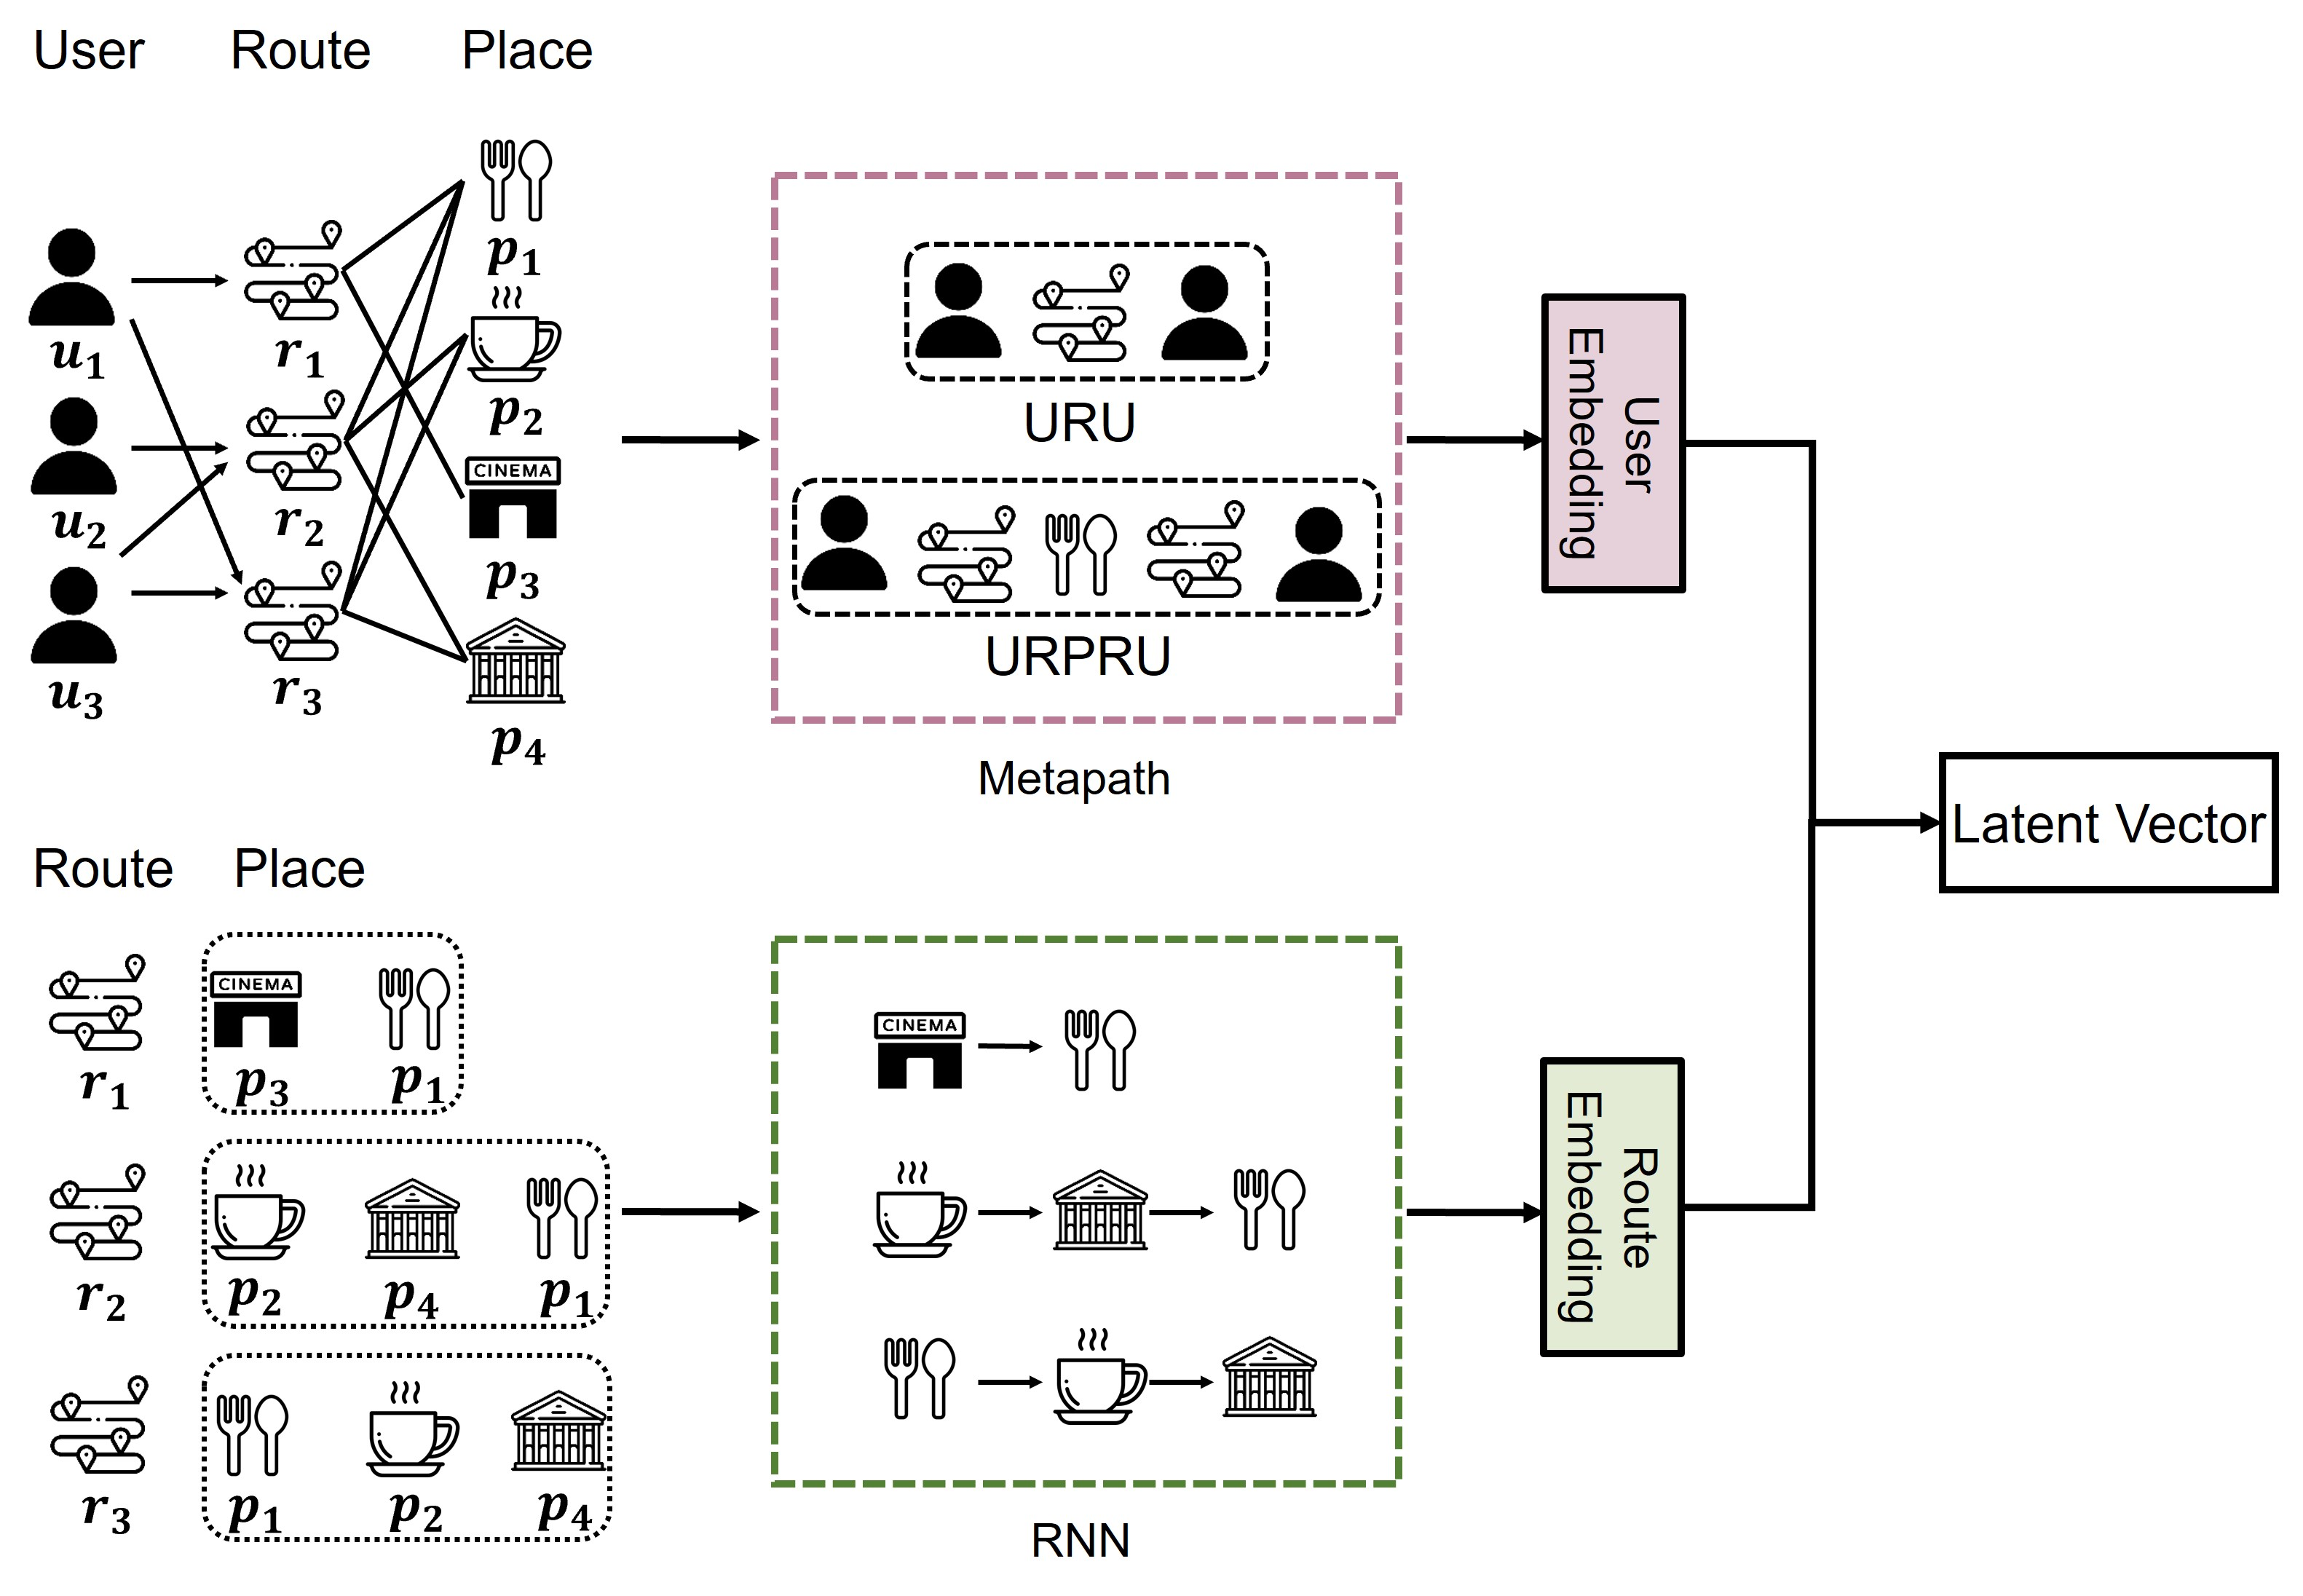
\includegraphics[width=1\linewidth]{fig/example.jpg}
	\hfil
	\caption{Example of embedding latent vector.}
	\label{fig2}
\end{figure}

\section{CGAN-based Route Recommendation}
\label{sec:Model}
This section describes the proposed travel route recommendation model in this study.

To address the problems introduced in Section \ref{sec:Intro}, our proposed model comprises three key components. 

First, we construct a latent vector to consider features of the relationship between users and routes, including places, and features of the routes represented by the sequence of places. 

Second, we utilize a Conditional Generative Adversarial Network (CGAN) to improve data sparsity issues related to the relationship between routes and users. We train the CGAN using the latent vector and preferences as inputs, generating samples from the generator. 

Lastly, we predict user route preferences using these generated samples with a Multilayer Perceptron (MLP). An overall schematic of the proposed approach is presented in Fig \ref{fig3}. The following subsections will detail these steps.

\subsection{Latent Vector Embedding}
The proposed model extracts features of the relationship between users and routes, including places, as well as features of routes represented by sequences of places. Then it constructs a latent vector through principal component analysis. The method for extracting features of the user and route is as follows.

\subsubsection*{User Embedding}

To model the relationship between users, routes, and locations, we adopt the use of Heterogeneous Information Networks (HIN) as a method for extracting user features. HINs are composed of various types of nodes and links, and their flexibility in modeling data heterogeneity has made them valuable in characterizing diverse auxiliary data for recommendation systems. We model an HIN composed of user nodes, route nodes, and location nodes. The connections between user nodes and route nodes represent interactions between users and routes, while the connections between route nodes and location nodes indicate the locations that make up a given route. For example, Fig \ref{fig1}(a) illustrates an example of a HIN for travel routes. This network comprises three types of nodes($i.e.$, Users (U), Routes (R), and Places (P)), and their interactive relationships. In this example, the HIN models the routes experienced by user $u_1$: route $r_1$ consisting of `cinema, restaurant' and route $r_3$ composed of `restaurant, café, museum'.

The approach adopts network embedding techniques to learn the relationships between HIN users and the places in the routes they have experienced. However, most network embedding methods primarily focus on homogeneous networks and aren't effective in modeling heterogeneous networks. Therefore, in this research, we utilize meta-path-based embedding methods. Metapaths are effective in capturing complex relationships between nodes in HINs. Considering the various characteristics and meanings reflected by meta paths, we generate node sequences using a meta path-derived random walk strategy to effectively learn user features. To effectively learn about the characteristics of the relationship between users and routes, including places, a meta path starting from the user node is designed to generate node sequences. For example, as shown in Fig \ref{fig2}, users and routes can be connected through various meta paths, each representing different meanings. The ‘User-Route-Place-Route-User (URPRU)’ path indicates users who have experienced routes composed of the same places. Meanwhile, the ‘User-Route-User (URU)’ path signifies users who have experienced the same route.


\subsubsection*{Route Embedding}

The routes are represented as sequences of locations, and the order of these locations is a critical factor among the features of a route. Taking Fig \ref{fig2} as an example, consider the `café - museum - restaurant' route, denoted as $r_2$, and the `restaurant – café - museum' route, denoted as $r_3$. These routes consist of the same locations but are defined as distinct routes by users due to the different order in which the locations appear. To leverage this sequential information, it is crucial to encode route data in a way that preserves the inherent order. 

In this paper, we utilize Recurrent Neural Networks (RNN) for route embedding. RNN, known for its ability to capture dependencies between sequential elements, is particularly well-suited for handling sequence data. We process the places that make up a route as a sequence of locations, encoding each place into a unique integer. To ensure all sequences have the same length, we perform padding set to the length of the longest route and use this as the input for the RNN. As shown in Fig \ref{fig2}, in our approach, we use RNN to preserve the continuity of routes, process information sequentially and consequently learn and embed route patterns. We use integer encoding and padded sequences as input for our routes. 
\begin{figure}[htb!]
	\centering
	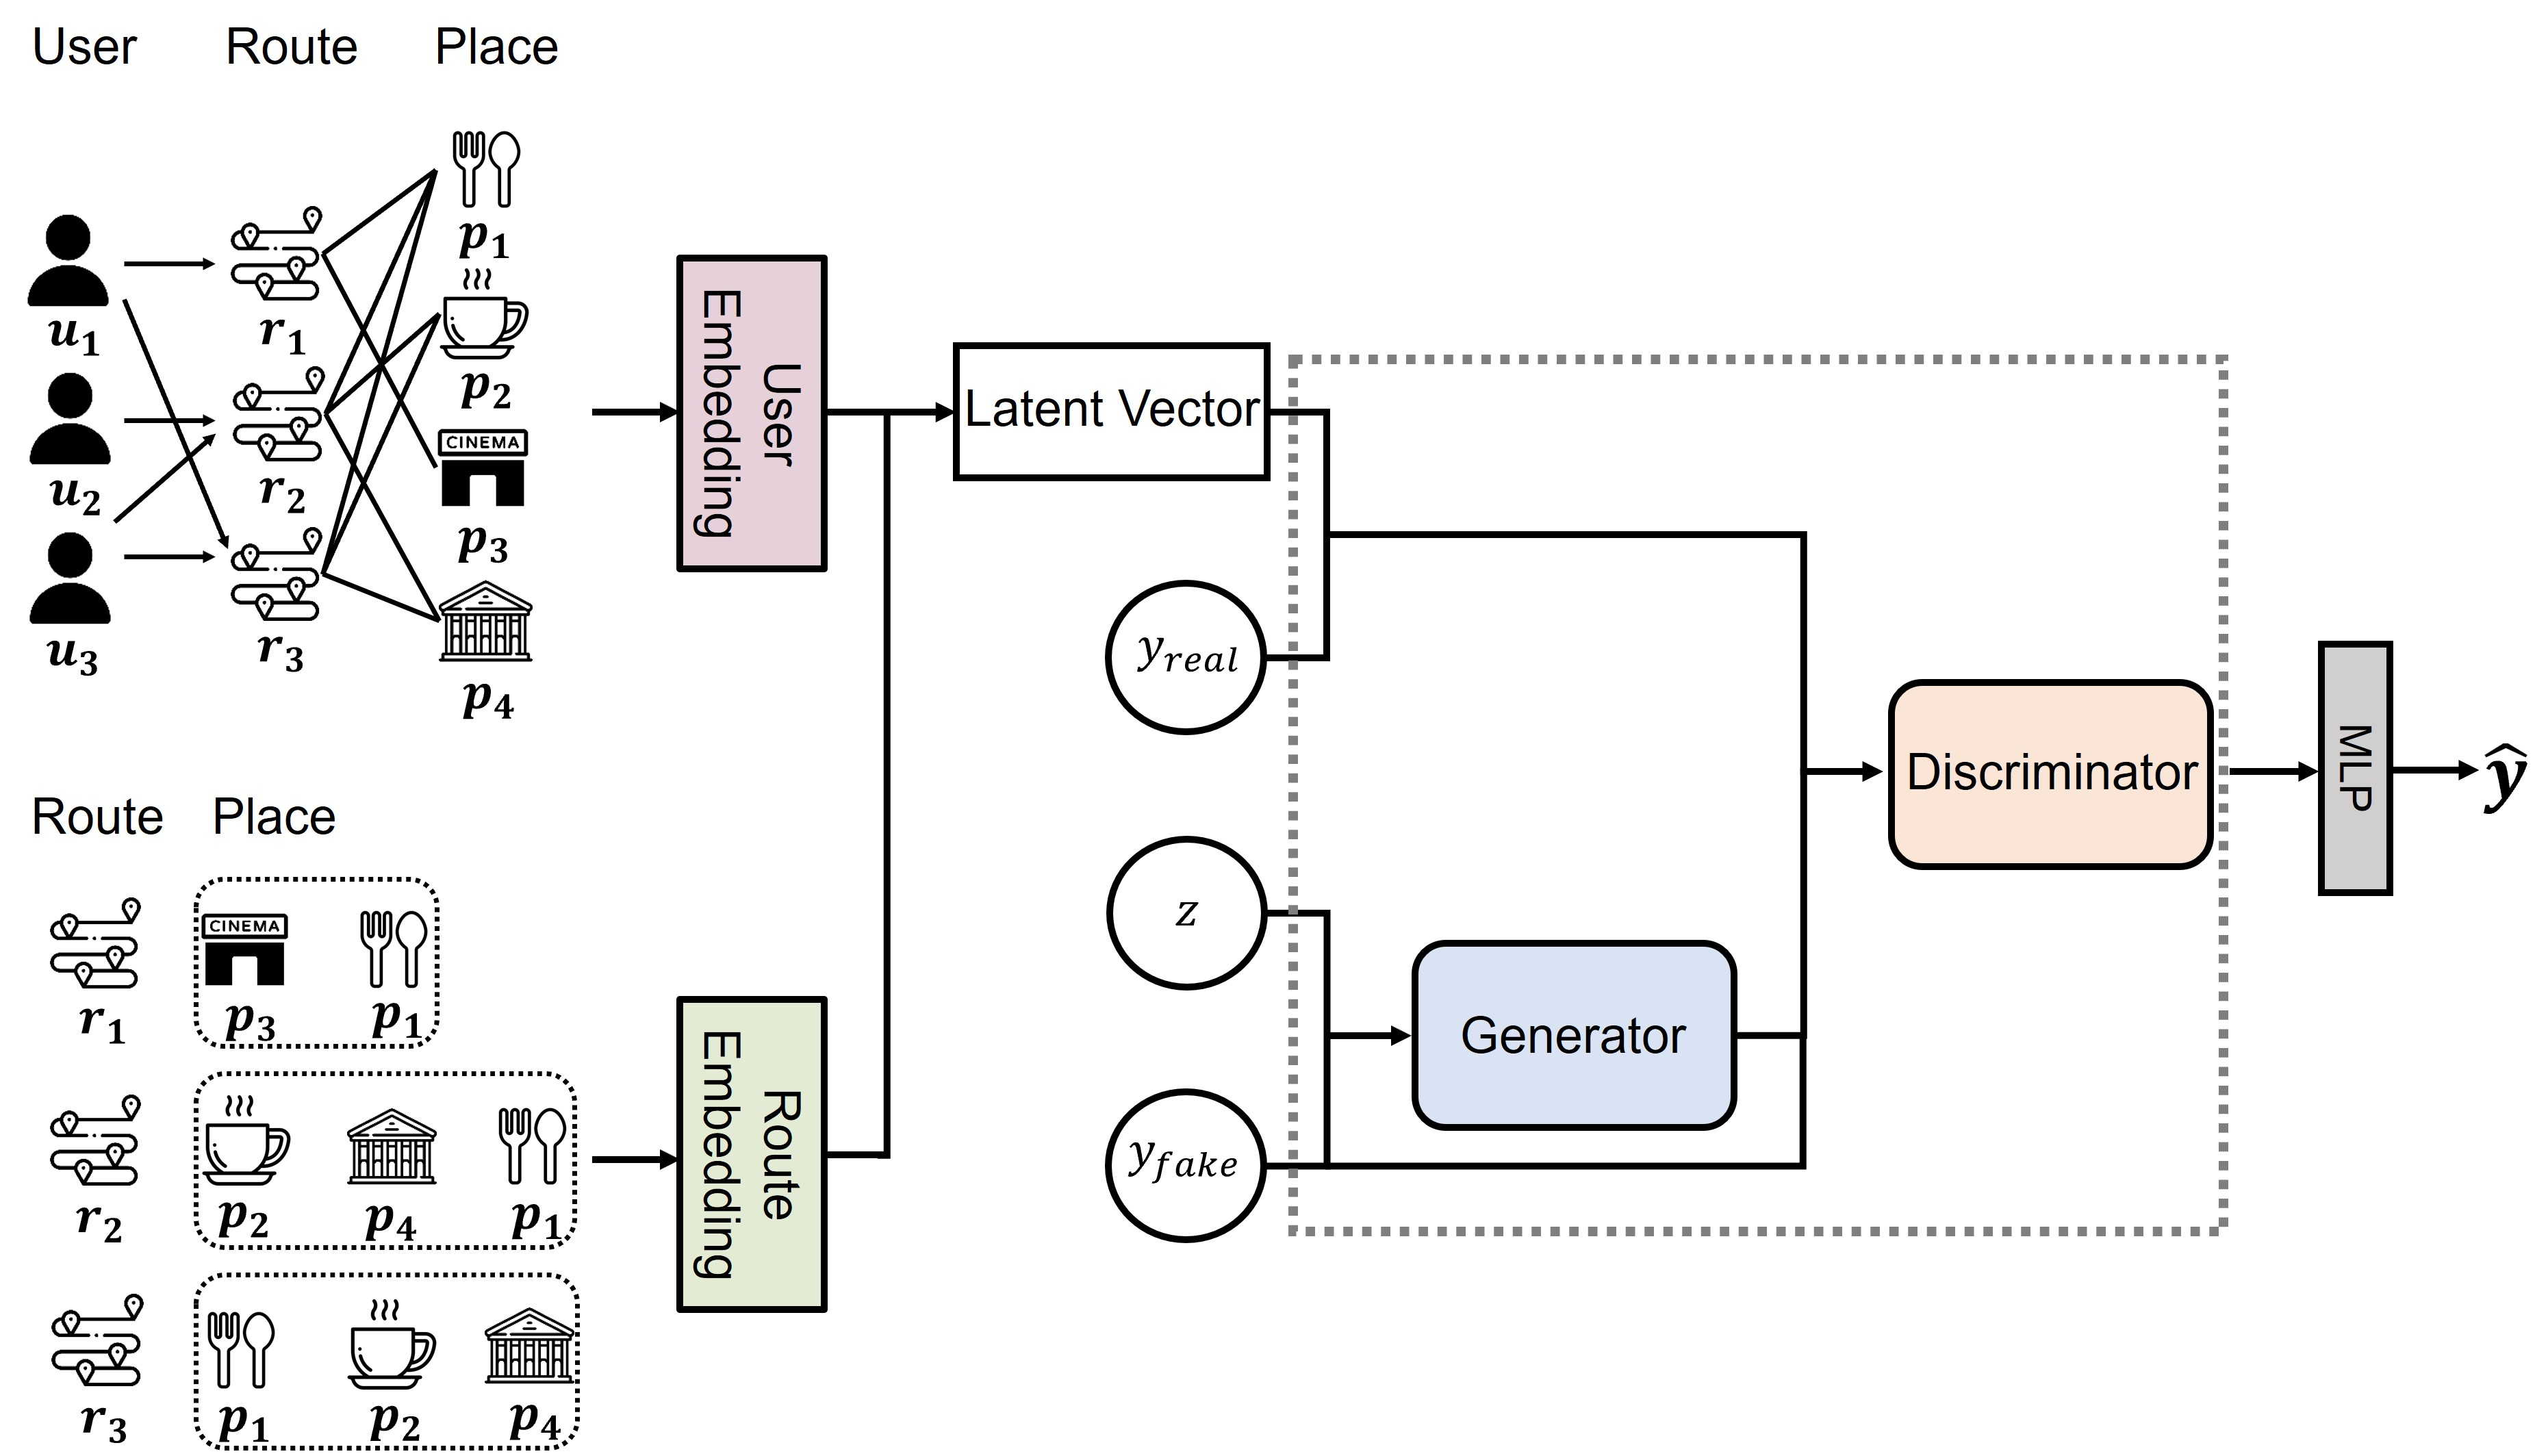
\includegraphics[width=1\linewidth]{fig/framework_5.jpg}
	\hfil
	\caption{Framework of the proposed model.}
	\label{fig3}
\end{figure}

\subsection{Latent Vector Augmentation}

In the previous step, a latent vector was constructed to consider the characteristics of the relationship between users and routes, including places, and the features of routes represented by sequences of places. This step explores how to train a Conditional Generative Adversarial Network (CGAN) using the latent vector to solve the data sparsity problem related between paths and users. CGAN is trained like a Generative Adversarial Network (GAN). GAN involves the generator and discriminator models competing adversarially with each other to learn and generate samples that resemble real data. The difference is that in CGAN, both the generator and discriminator consider conditional information y. This study adopts the latent vector and user preferences regarding routes as the conditional information $y^c$ for CGAN's input data. Once trained, CGAN produces samples with features similar to the input data from its generator. The CGAN used in this paper is defined as follows:\\
\begin{equation}
	\min_G \max_D V(G, D) = E_G + E_D
\end{equation}
\\
The objective function of CGAN can be formulated as a minimax problem, with $E_D$ and $E_G$ denoting the objective functions of the discriminator and the generator, respectively.\\
\begin{equation}
	E_G = \mathbb{E}_{z \sim p_z(z)}[\log(1 - D(G(z|y^c)))]
\end{equation}
\\
$Pz$ represents the distribution of noise, and $z$ represents a noise sample drawn from this $Pz$ distribution. $G$ represents the generator, and $G(z)$ represents the synthetic data generated by the generator using the random noise $z$. The generator's goal is to produce generated samples that can deceive the discriminator into believing they are real data.\\
\begin{equation}
	E_D = \mathbb{E}_{x \sim p_{\text{data}}(x)}[\log D(x|y^c)]
\end{equation}
\\
$p_{\text{data}}$ represents the distribution of latent vectors, where $x$ denotes a sample drawn from this $p_data$ distribution. $D(x|y^c)$ represents the probability that the discriminator accurately distinguishes generated samples, considering the condition $y$, from real data. When the input data corresponds to a latent vector with actual preferences, $D(x|y^c)$ yields an output of 1. In contrast, if it is identified as synthetic data, it returns an output of 0. The primary objective of the discriminator is to set $D(x|y^c)$ to 1 while keeping $D(G(z|y^c))$ at 0.

The discriminator strives to effectively differentiate between $D(x|y^c)$ and $G(z|y^c)$. Consequently, $D(x|y^c)$ is designed to be 1, and $D(G(z|y^c))$ is designed to be 0. The discriminator's learning process aims to ensure that the value of $log(1 - D(G(z)))$ equals 0. On the other hand, the generator's objective is to make the discriminator perceive $G(z|y^c)$ as real data. Therefore, $D(G(z|y^c))$ is intended to be 1, and $log(1 - D(G(z|y^c)))$ is optimized to achieve its maximum value. Ultimately, the discriminator $D$ seeks to maximize $V(D, G)$, while the generator $G$ strives to minimize $V(D, G)$ during the learning process.


\subsection{Route Recommendation}
To address the data sparsity issue related to routes and user relationships, this study utilized latent vectors and preferences as input data for a CGAN. The generator produces samples with characteristics similar to the input data. For predicting user route preferences, this research adopts a Multilayer Perceptron (MLP). An MLP is a neural network composed of multiple layers, useful for capturing nonlinearity and learning complex interactions between various features. It can be defined as follows.\\
\begin{equation}
	\centering
	\begin{gathered}
		h_1 =\sigma(W_1 \cdot X + b_1) \\
		h_2 =\sigma(W_2 \cdot h_1 + b_2) \\
		\vdots \\
		h_k =\sigma(W_k \cdot h_{k-1} + b_k) \\
		\hat{y} =\sigma(W_{\text{out}} \cdot h_k + b_{\text{out}})
	\end{gathered}
\end{equation}
\\
The input vector $X$ comprises a combination of the latent vector of the generated sample and the user's preference. $k$ represents the number of hidden layers, and each hidden layer comprises a linear transformation and an activation function. The activation function, denoted as $σ$, employs ReLU. $h_k$ represents the output of the k-th hidden layer, where $W_k$ represents the weight matrix, and $b_k$ denotes the bias vector. The output of the final hidden layer serves as the prediction, \(\hat{y}\) representing the user's predicted preference. The loss function is defined as in Equation \ref{equation8}.\\
\begin{equation}
	\mathcal{L} = \frac{1}{n} \sum_{i=1}^{n} (y_i - \hat{y}_i)^2
	\label{equation8}
\end{equation}
\\
In this paper, Our objective is to predict users' preferences (from 1 to 5) for routes. To achieve this, the Mean Squared Error (MSE) is employed as the loss function. In this context, $N$ represents the number of data samples, $y_i$ denotes the actual preference ratings of the users, and $\hat{y}_i$ signifies the predicted values by the model. Additionally, the Stochastic Gradient Descent (SGD) algorithm is utilized to optimize the model. This involves calculating the gradient of the loss function to appropriately update the model's weights and biases.

\begin{comment}
	$z, \quad y$\\
	$e = \begin{bmatrix} z \\ y \end{bmatrix}$\\
	$\hat{y} = \sigma(MLP(e))$...
\end{comment}






\section{Experiments}
\label{sec:Exe}
In this section, we demonstrate the effectiveness of the proposed model by comparing it with four other recommendation methods using real-world datasets.

\subsection{Datasets}
For our experiments, we utilized real datasets: TripAdvisor tour package datasets. Detailed statistics of datasets can be found in Table \ref{sec6:data}.
\begin{table}[htb!]
	\centering
	\setlength{\tabcolsep}{12pt}
	\renewcommand{\arraystretch}{1.4}
	\caption{Summary of datasets statistics.}
	\label{sec6:data}
	\begin{tabular}{@{}ccccc@{}}
		\toprule
		Datasets    & Users  & Routes & Places & Ratings \\
		\midrule
		TripAdvisor & 12,886 & 628    & 666    & 15,004  \\
		\bottomrule 
	\end{tabular}
\end{table}

\textbf{TripAdvisor}. We collected tour package and review data from TripAdvisor\footnote{https://www.tripadvisor.com/}, a renowned review platform in the tourism sector. TripAdvisor's tour packages include various tourist attractions and activities organized into itineraries. For simplicity, we consider these tour packages as routes and the itineraries as places. Users rate these tour packages on a scale of 1 to 5 and leave reviews, allowing travelers to reference these reviews and ratings to choose suitable tour packages for themselves. In our data collection, we focused on tour packages in South Korea. We excluded packages with only one place or spanned multiple days, resulting in a dataset of 628 tour packages and 666 places, along with 15,004 review data entries. The tour packages in our dataset vary, containing anywhere from a minimum of 2 to a maximum of 18 places

Using the TripAdvisor datasets, we modeled a Heterogeneous Information Network (HIN) consisting of three types of nodes: users, routes, and places. For this work, focusing on user preferences, we classified ratings of 4-5 stars as 1 (like) and the rest as 0 (dislike) for experimental purposes. 


\subsection{Experimental Setup}

\subsubsection*{Parameters Settings}
The proposed model is implemented using Python 3.10 and Scikit-learn 1.2.2. For the RNN, TensorFlow 2.11.0 is used, and CGAN is implemented through keras 2.11 In HIN embedding, Metapath2vec is set with a walk length of 50, a repeat count \(n\) of 10, and an embedding size of 128. The RNN utilizes an LSTM layer with embedding units. The dimension for principal component analysis is set to 128. CGAN is configured with 500 epochs, a learning rate of 0.01, and a batch size of 128. The training-testing ratio is set as 0.8, 0.2.

\subsubsection*{Methods to compare}
To evaluate the performance of our proposed approach, we compared it with three baseline models:\\

\begin{itemize}
	\item FM \cite{5694074}: Factorization Machines (FM) pairwise interactions between features in a dataset (including user, item, and contextual features) using the dot product of latent vectors associated with each feature. They are widely used in recommender systems to capture complex relationships and improve prediction accuracy.
	
	\item DeepFM \cite{Guo2017}: DeepFM combines Factorization Machines (FM) with deep neural networks (DNNs) to learn both low-order (pairwise) and high-order (complex) feature interactions. The FM component captures pairwise interactions, while the DNN component models non-linear relationships. DeepFM is widely used in personalized recommendation systems, leveraging information like user behavior, preferences, item features, and contextual data to provide tailored suggestions.
	
	\item NeuMF \cite{10.1145/3038912.3052569}: Neural Matrix Factorization(NeuMF) is a recommendation system model that extends traditional Matrix Factorization (MF) by incorporating a neural network architecture to model the interaction between users and items.

	\item NFM \cite{10.1145/3077136.3080777}: Neural Factorization Machines(NFM) is a method based on deep learning for item recommendation, combining a hidden layer inspired by Generalized Matrix Factorization (GMF) and a Multi-Layer Perceptron (MLP) to learn the user-item interaction function. NFM is primarily used for modeling the interaction between users and items, enabling effective personalized recommendations.
	
\end{itemize}

\subsubsection*{Evaluation Metric}
The primary aim of this study is to predict users' preferences for routes. Consequently, we employ MAE (Mean Absolute Error) and RMSE (Root Mean Squared Error) to assess the performance of the recommendations. The metrics MAE and RMSE are defined as follows:\\
\begin{equation}
	MAE = \frac{1}{N} \sum_{i=1}^{N} |y_i - \hat{y}_i|
\end{equation}
\\
\begin{equation}
	RMSE = \sqrt{\frac{1}{N} \sum_{i=1}^{N} (y_i - \hat{y}_i)^2}
\end{equation}
\\
$N$ represents the number of ratings in the test set, $y_i$ is the actual rating given by a user to a route, and $\hat{y}_i$ is the predicted rating from a model. As indicated by the definition, a lower value of MAE or RMSE signifies better performance.



\subsection{Experiments Results}
\subsubsection{Evaluation}
This experiment validates the performance of the proposed model in route recommendation by comparing it with other recommendation methods. The total rating records for each dataset were divided into training and test sets for the experiment. The TripAdvisor dataset has relatively abundant review data, the training set was set to 60\% and the test set to 40\% for the experiment. The results of the datasets regarding MAE and RMSE are presented in Table \ref{sec6:results1}. The major findings from the experimental results can be summarized as follows:

\begin{table}[htbp!]
	\centering
	\setlength{\tabcolsep}{12pt}
	\renewcommand{\arraystretch}{1.4}
	\caption{Compare the performance of route recommendation for different datasets.}
	\label{sec6:results1}
	\begin{tabular}{ccccc}
		\toprule
		\multirow{2}{*}{Method} & \multicolumn{2}{c}{TripAdvisor} \\
		& MAE             & RMSE           \\
		\midrule
		FM                      & 0.3845          & 0.5515            \\
		DeepFM                  & 0.2953          & 0.5051      	\\
		NFM                     & 0.3822          & 0.5058      \\
		NeuMF                   & 0.3370          & 0.5071       \\
		\textbf{Proposed}       & \textbf{0.1439} & \textbf{0.3320} \\
		\bottomrule
	\end{tabular}
\end{table}

\begin{enumerate}
	\item The proposed model achieves the best performance in both datasets in terms of MAE and RMSE. In the TripAdvisor dataset, the proposed model recorded an MAE of 0.0993 and an RMSE of 0.2430. This represents an improvement of approximately 197.34\% and 107.86\% compared to DeepFM, and an improvement of 239.36\% in MAE and 108.72\% in RMSE compared to NeuMF, which previously showed the best performance.
		
	\item Compared to the traditional method, FM, neural network-based methods (DeepFM, NFM, NeuMF) showed greater improvements in terms of MAE and RMSE. These results indicate that neural network-based methods can more precisely capture users' preferences and the characteristics of routes in recommendations, thereby providing more accurate suggestions.
	
	\item The proposed model utilizes a latent vector that considers user characteristics and route features, using HIN and RNN. Compared to methods that learn user and route interactions separately, the latent vector effectively captures the features of both users and routes, demonstrating its effectiveness in the route recommendation process.
	
	\item The results indicate that using the samples generated by the proposed model is effective in addressing sparse data problems and improving predictions in scenarios such as travel route recommendations.
\end{enumerate}



\subsubsection{Performance Comparison of Data Sparsity}
In the previous section, we demonstrated that the proposed model improves predictions in sparse datasets. In this section, we extend these experiments to verify the proposed model’s adaptability in sparse data environments. We utilized the TripAdvisor dataset, which has a relatively abundant amount of review data. We set the training set proportions to four different percentages \{20\%, 40\%, 60\%, 80\%\} and compared the adaptability of various models at each training set proportion using MAE and RMSE. The experimental results are presented in Fig \ref{sec6:results2}.

\begin{figure}[!htbp]
	\centering
	\begin{subfigure}[b]{0.495\textwidth}
		\centering
		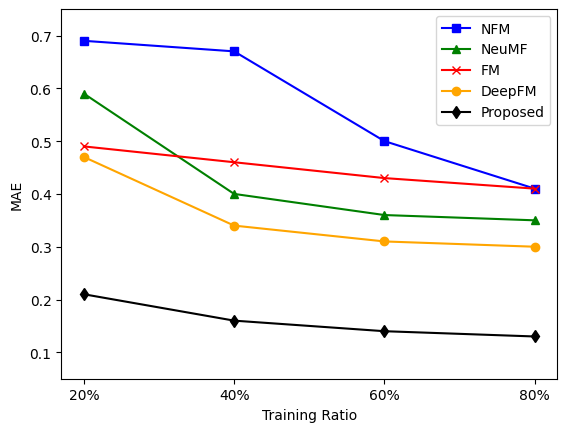
\includegraphics[width=\textwidth]{fig/Training_MAE.png}
		%\caption{MAE}
		\label{fig:image1}
	\end{subfigure}
	\hfill
	\begin{subfigure}[b]{0.495\textwidth}
		\centering
		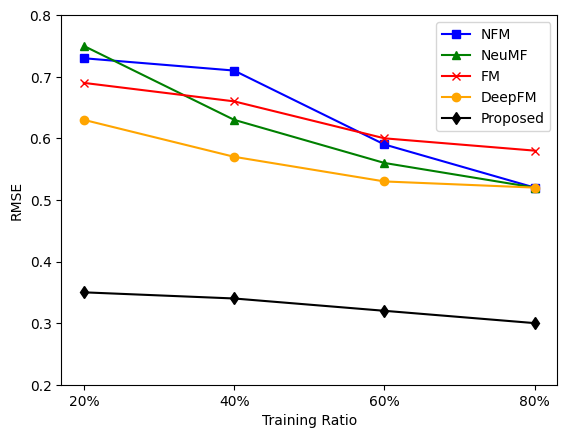
\includegraphics[width=\textwidth]{fig/Training_RMSE.png}
		%\caption{RMSE}
		\label{fig:image2}
	\end{subfigure}
	\caption{Compare the performance of route recommendation for train ratio.}
	\label{sec6:results2}
\end{figure}


According to the experimental results, the proposed model demonstrated superior performance compared to other models, even in sparse data environments. Observing the performance changes of the recommendation model according to the proportion of data, most recommendation models tend to improve in performance as the amount of training data increases. The most notable result appears in the sparsest data environment. In this environment, the proposed model exhibited the best performance and recorded an improvement of approximately 0.16 in MAE and 0.19 in RMSE compared to DeepFM, which showed the best performance. This represents an improvement of about 197.34\% and 107.86\%, respectively. These results emphasize the proposed model's adaptability in sparse data environments and highlight the usefulness of utilizing generated samples.

Through this experiment, the proposed method using generated samples with Latent vectors has proven effective in sparse data environments. Such results suggest that using the proposed model can improve predictive performance even in sparse travel route recommendation scenarios.


\subsubsection{Comparative Analysis: CGAN vs. Non-CGAN Approaches}

In this section, we delve into a comparative analysis of model performance with and without the integration of Conditional Generative Adversarial Networks (CGANs). We maintain the experimental setup from the previous section, systematically increasing the test dataset proportion to \{20\%, 40\%, 60\%, 80\%\}. The results obtained from both scenarios are then juxtaposed to highlight the impact of CGANs, specifically focusing on the Root Mean Square Error (RMSE) metric.

Our findings unequivocally demonstrate the superior performance of models incorporating CGANs across all tested dataset proportions. The inclusion of CGANs consistently yields significantly lower RMSE values compared to the non-CGAN counterparts. This underscores the pivotal role of CGANs in enhancing the model's ability to learn and generalize from the data, ultimately leading to more accurate predictions. The results of these experiments are presented in Figure \ref{fig4}

\begin{figure}[!htbp]
	\centering
	\begin{subfigure}[b]{0.495\textwidth}
		\centering
		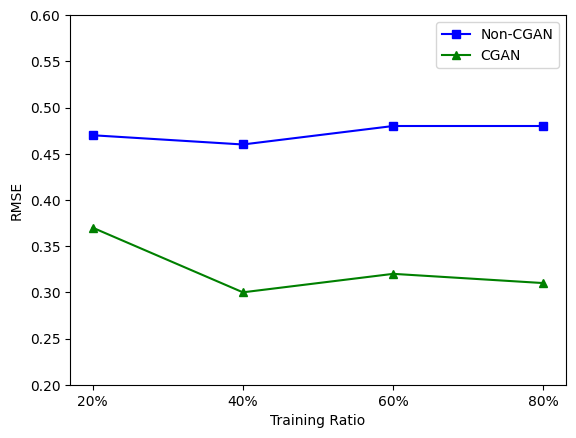
\includegraphics[width=\textwidth]{fig/compare_without_include_CGAN.png}
		\label{fig4:image1}
	\end{subfigure}
	\hfill
	\caption{Compare the results of CGAN vs. Non-CGAN}
	\label{fig4}
\end{figure}

The observed performance gains with CGANs, as reflected in the reduced RMSE values, can be attributed to several key factors:

\begin{itemize}
	\item Enhanced Data Generation: CGANs excel at generating synthetic data samples that closely resemble the real data distribution. This augmented dataset aids in addressing issues like data scarcity and class imbalance, thereby improving the model's learning capacity and reducing prediction errors.
	
	\item Improved Feature Representation: CGANs contribute to learning richer and more informative feature representations. By conditioning the generation process on specific attributes or labels, CGANs enable the model to capture intricate relationships within the data, leading to more accurate predictions and lower RMSE values.

	\item Regularization Effect: The adversarial training process inherent in CGANs acts as a form of regularization, preventing overfitting and promoting better generalization to unseen data. The generator and discriminator networks in CGANs constantly challenge each other, forcing the model to learn robust representations that are less prone to errors.

	\item Addressing Domain Shift: In scenarios where the training and test data distributions differ, CGANs can help bridge the gap by generating synthetic samples that align with the target domain. This mitigates the negative effects of domain shift and improves the model's adaptability, leading to more consistent and accurate predictions across different data distributions.
\end{itemize}

In conclusion, the integration of CGANs proves to be a critical factor in achieving superior model performance, as evidenced by the high RMSE values observed in our experiments. The ability of CGANs to generate high-quality synthetic data, learn informative representations, regularize the training process, and address domain shifts collectively contributes to their significant impact on model effectiveness and accuracy.

The results of our experiments strongly advocate for the inclusion of CGANs in similar machine-learning tasks to unlock their full potential and minimize prediction errors.

\subsubsection{Usability of Generated Samples}
In the previous phase, two experiments confirmed that the proposed model uses the generated samples effectively in sparse data environments and improves predictive performance. In this study, we evaluate whether the actual generated samples are sufficient for improved recommendation performance. Therefore, we use the generated Sample Dataset (SD), the Original Dataset (OD), and the Augmented Dataset (AD) combining SD and OD as training sets to predict user preferences for routes via MLP. As with previous experiments, we set the training set at 60\% and the test set at 40\%. The results are presented in Table \ref{sec6:results4}.

Experimental results demonstrate that predictions made solely using generated data show similar performance in terms of MAE and RMSE when compared to existing methods outlined in Table \ref{sec6:results1}. 
The experimental results demonstrate that while the Augmented Dataset (AD) performance in terms of RMSE and MAE is not as good as the Original Dataset (OD), it still yields sufficiently usable results. This indicates that the Augmented Dataset can be employed effectively as training data.

However, the performance of the Sample Dataset (SD) suggests a need for further parameter adjustments and improvements. Specifically, the values for the Sample Dataset highlight the necessity to refine the generation process to enhance the quality of the synthetic samples.

These results validate the effectiveness of the generated samples and confirm that the Augmented Dataset can be used as training data. This finding suggests the possibility of developing effective recommendation systems even in environments with limited data availability.

\begin{table}[!htbp]
	\centering
	\setlength{\tabcolsep}{12pt}
	\renewcommand{\arraystretch}{1.4}
	\caption{Performance on OD, SD, and AD.}
	\label{sec6:results4}
	\begin{tabular}{ccc}
		\toprule
		Data & MAE    & RMSE   \\
		\midrule
		OD   & 0.0458 &  0.1709 \\
		SD   & 1.2181 & 1.4171 \\
		AD   & 0.1178 & 0.3881 \\
		\bottomrule
	\end{tabular}
\end{table}

\subsubsection{Effect of Sample Number}
In this study, we conduct experiments on the influence of the number of samples generated by the generator, denoted as $K$. This experiment analyzes the performance concerning the number of samples created utilizing latent vectors.

Since the TripAdvisor datasets have different sparsity levels, we set different initial values for the $K$ dataset. The TripAdvisor dataset had its initial value of $K$ set to about one-third of the original data size, which is 5000. The performance based on the number of samples $K$ was measured using MAE.
\begin{figure}[!htbp]
	\centering
	\begin{subfigure}[b]{0.495\textwidth}
		\centering
		\includegraphics[width=\textwidth]{fig/Tripadvisor_K.png}
		\label{fig5:image1}
	\end{subfigure}
	\hfill
	\caption{Effect of Sample Size.}
	\label{fig5}
\end{figure}

The results, as shown in Fig \ref{fig5}, indicate that for the TripAdvisor dataset, the model achieved optimal performance when $K$ was approximately 5,000, with performance declining thereafter. Specifically, after reaching 5,000 samples, the model's performance, measured by MAE, increased, indicating a decrease in accuracy. Following this decline, performance improved again around 20,000 samples, before experiencing another decline and subsequent improvement. This pattern of fluctuating performance highlights the non-linear relationship between the number of samples and model accuracy. The ratio of the optimal $K$ value to the size of the original data was observed to vary across datasets. In the relative review-rich Tripadvisor dataset, the model performed best when generating samples approximately 3 times the size of the original data.

These experimental results suggest that increasing the $K$ value does not necessarily lead to a linear improvement in model performance. In sparse datasets, in particular, performance is more sensitive to changes in the number of samples. This further implies that the optimal $K$ value may be influenced by the sparsity of the dataset.

\section{Conclusion \& Future Work}
\label{sec:Con}

This study proposes a novel technical and domain-specific methodology to address the challenges of route recommendation. The proposed method leverages latent vectors to effectively capture the characteristics of user-route relationships, incorporating information about places and routes represented as a sequence of places. To mitigate data sparsity in user-route relations, a Conditional Generative Network (CGAN) is employed.

A Heterogeneous Information Network (HIN) is utilized to model the complex relationships between users, their experienced routes, and places. User features are extracted using a meta-path-based embedding approach, while Recurrent Neural Networks (RNN) extract features from routes represented as a sequence of places. Latent vectors are constructed by combining user and route features and applying principal component analysis. The CGAN is trained using these latent vectors and user route preferences as conditional information to address the data sparsity issue. The generator, implemented as a Multilayer Perceptron (MLP), generates samples to predict user route preferences.

The performance of the proposed model is evaluated using real-world route datasets and compared with four other recommendation models using Mean Absolute Error (MAE) and Root Mean Squared Error (RMSE). In experiments designed to assess the performance difference between the proposed model and conventional methods, the proposed model demonstrated improvements of up to approximately 239.36\% and 108.72\% in MAE and RMSE, respectively, compared to the best-performing baseline model. Two additional experiments were conducted to investigate the adaptability of the proposed model in sparse data environments and to analyze the impact of the number of generated samples.

In the sparsest data environment, the proposed model exhibited improvements of about 197.34\% in MAE and 107.86\% in RMSE compared to the best-performing baseline model, confirming its robustness in handling sparse data.

Finally, an experiment to understand the influence of the number of generated samples revealed that the model's performance does not increase linearly with the number of samples, and the optimal number of samples varies depending on the sparsity level of the dataset.

Future work will address the limitations of this study and explore research directions to enhance the contributions presented in this paper.
\begin{itemize}
	\item Research incorporating additional route features: This study focused on the relationship between users and routes, examining features of routes represented as sequences of places. Incorporating additional features such as the atmosphere of places, distance between places, and total duration of the route could further refine personalized route recommendations.
	
	\item Research for general domain application: Our proposed model, specifically designed for route recommendation, may not be directly applicable to general recommendation domains such as books or movies. To address this limitation, future research could explore modifying or expanding the recommendation process of our model to enhance its applicability to diverse domains.
	
	\item Optimizing the generation and selection of samples: Given the non-linear relationship between sample size and performance, future research should investigate methods to optimize the generation and selection of samples. This could involve developing adaptive sampling techniques that adjust the number and quality of generated samples based on specific characteristics of the dataset. Additionally, exploring different sampling strategies, such as importance sampling or stratified sampling, could help further improve the generated samples' effectiveness.

	\item Investigating the impact of sample quality on performance: While this study focused on the quantity of samples, the quality of generated samples also plays a crucial role in model performance. Future research could investigate the impact of sample quality on recommendation accuracy and explore techniques to improve the realism and informativeness of generated samples. This could involve refining the generation process, incorporating domain knowledge, or utilizing feedback mechanisms to enhance sample quality iteratively.
\end{itemize}

By addressing these limitations and exploring these future directions, this research can contribute to the advancement of personalized recommendation systems, particularly in scenarios with limited data availability.




\bibliographystyle{unsrt} 
\bibliography{library}

\end{document}


